\documentclass[11pt,aspectratio=169]{beamer}
% WiL progress update, 22 October 2026.  One claim per slide, with the data
% that shows it on the same slide.  Figures are the project's own.
\usetheme{default}
\usecolortheme{seagull}
\setbeamertemplate{navigation symbols}{}
\setbeamertemplate{footline}[frame number]
\setbeamerfont{frametitle}{size=\large,series=\bfseries}
\setbeamercolor{frametitle}{fg=black!85}
\usepackage[T1]{fontenc}
\usepackage[utf8]{inputenc}
\usepackage{booktabs}
\usepackage{siunitx}
\usepackage{graphicx}
\usepackage{xcolor}
\usepackage{tikz}
\usetikzlibrary{arrows.meta,positioning,shapes.geometric,fit,calc}
\sisetup{detect-all,range-phrase=--,range-units=single}
\newcommand{\repo}[1]{\texttt{\detokenize{#1}}}
\newcommand{\FIG}{../../final_report/figures}
\newcommand{\OUT}{../../../../output/compare/simulation}
\newcommand{\src}[1]{\vfill{\tiny\color{black!55}Source: #1}}
\definecolor{neg}{HTML}{B00020}

\title{WiL update, 22 October 2026}
\subtitle{Realistic world \textperiodcentered\ Experiment insights \textperiodcentered\ Motion gate}
\author{Bolton Athit Davies}
\date{}

\begin{document}

\begin{frame}
  \titlepage
\end{frame}

\begin{frame}{Contents}
  \begin{enumerate}
    \item Realistic world
    \item Experiment insights
    \item \repo{filter_mode:=motion}: why it does not work
  \end{enumerate}
\end{frame}

% ===================================================================== Part 1
\section{Realistic world}
\begin{frame}{1. Warehouse flow shapes in the design literature}
  \centering
  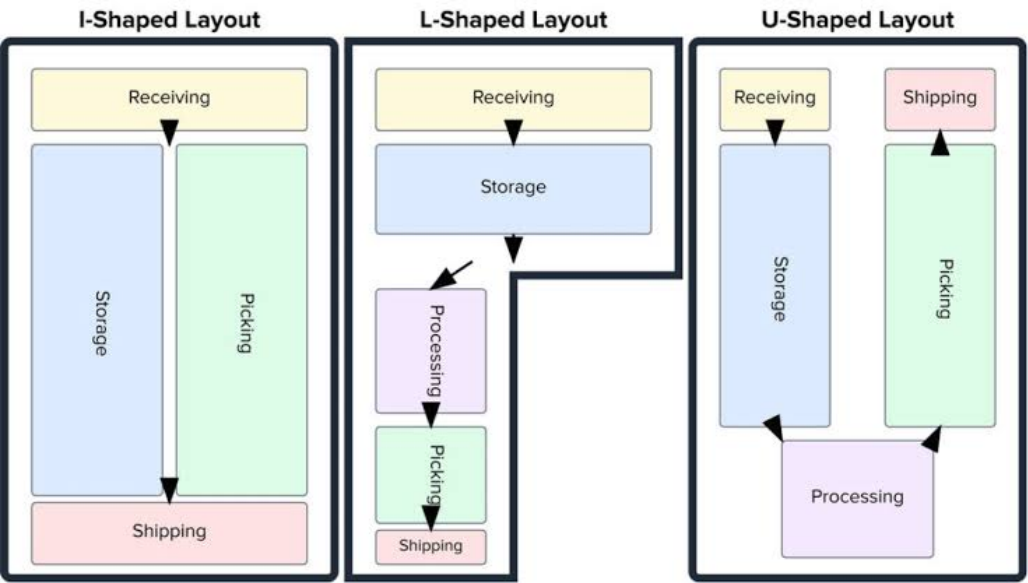
\includegraphics[height=0.72\textheight]{warehouse_flow_shapes.png}
  \par{\footnotesize Three canonical layouts: I-shape (through flow), L-shape, U-shape. The realistic worlds implement the \textbf{I} and the \textbf{U}; the L was not generated.}
\end{frame}

\begin{frame}{1. U-shape layout: receiving and dispatch share the north wall}
  \centering
  \includegraphics[height=0.78\textheight]{\FIG/plan_realistic_u.png}
  \par{\footnotesize Filled rectangles: 126 objects by zone \textperiodcentered\ coloured lines: 4 carrier routes \textperiodcentered\ dashed green: 4 people \textperiodcentered\ grey: recorded route of \repo{dynamic_00_000}}
\end{frame}

\begin{frame}{1. I-shape layout: receiving north, dispatch south}
  \centering
  \includegraphics[height=0.78\textheight]{\FIG/plan_realistic_i.png}
  \par{\footnotesize 121 objects \textperiodcentered\ same carriers and people \textperiodcentered\ the grey recorded route crosses the racks here, so the I recordings use a new route}
\end{frame}

\begin{frame}{1. Four recordings: one per layout and twin, routes hand-driven}
  \begin{columns}[T]
    \column{0.55\textwidth}
      \scriptsize\setlength{\tabcolsep}{3pt}
      \begin{tabular}{lllrrr}
        \toprule
        Recording & Layout & Traffic & Objects & Route [m] & Span [s] \\
        \midrule
        \repo{realistic_000} & U & no & 125 & 171 & 126 \\
        \repo{realistic_001} & I & no & 119 & 133 & 97 \\
        \repo{realistic_002} & U & yes & 125 & 103 & 80 \\
        \repo{realistic_003} & I & yes & 119 & 158 & 117 \\
        \bottomrule
      \end{tabular}
      \vspace{0.8em}
      \footnotesize
      \begin{itemize}
        \item Same object count within a layout (125 / 119): the twin differs only in whether the 4 carriers move
        \item Route column: the U pair differs by \SI{68}{\metre}, so on U a static-vs-traffic difference mixes route with traffic
      \end{itemize}
    \column{0.45\textwidth}
      \centering
      \includegraphics[width=0.48\textwidth]{\FIG/scene_allsensor_realistic_000.png}
      \includegraphics[width=0.48\textwidth]{\FIG/scene_allsensor_realistic_002.png}\\
      {\scriptsize \repo{000} U, no traffic \quad \repo{002} U, traffic}\\[0.5ex]
      \includegraphics[width=0.48\textwidth]{\FIG/scene_allsensor_realistic_001.png}
      \includegraphics[width=0.48\textwidth]{\FIG/scene_allsensor_realistic_003.png}\\
      {\scriptsize \repo{001} I, no traffic \quad \repo{003} I, traffic}
  \end{columns}
  \src{\repo{final_report/tables/dataset_scenes.tex}; blue trace = ground-truth route}
\end{frame}

\begin{frame}{1. When the traffic was actually in the camera: 37 \% of tracked time}
  \begin{columns}[T]
    \column{0.36\textwidth}
      \footnotesize
      \begin{itemize}
        \item Violet bands: a carrier or carried load within \SI{20}{\metre}, within $\pm\SI{45}{\degree}$, line of sight clear, from the bag's pose stream
        \item Grey bands: robot turning ($>$\SI{10}{\degree\per\second})
        \item Median violet share over the tracked runs: \SI{37}{\percent}
        \item People are not in the pose stream: no band for them
      \end{itemize}
    \column{0.64\textwidth}
      \includegraphics[width=\textwidth,height=0.82\textheight,keepaspectratio]{\OUT/exp3-insights/fig_traffic_timeline_lever0p338_light.png}
  \end{columns}
\end{frame}

% ===================================================================== Part 2
\section{Experiment insights}

\begin{frame}{2. Scoring bug: every ATE curve bottoms out at the \SI{0.338}{\metre} lever arm}
  \begin{columns}[T]
    \column{0.42\textwidth}
      \footnotesize
      \begin{itemize}
        \item Ground truth = model origin; both estimators report the IMU, \SI{0.338}{\metre} ahead in \repo{model.sdf}
        \item Figure: each line is one tracked run re-scored with the ground truth moved forward by $L$; the minima sit at the dotted line
        \item Median $L^{*}$ = \SI{0.34}{\metre}, IQR 0.32--0.40, 30 runs, both estimators, both worlds
      \end{itemize}
      \scriptsize
      \begin{tabular}{llrr}
        \toprule
        Static ATE [m] & & $L=0$ & $L=0.34$ \\
        \midrule
        extreme & VINS & 0.32 & \textbf{0.10} \\
        extreme & ORB & 0.37 & \textbf{0.19} \\
        realistic & VINS & 0.37 & \textbf{0.25} \\
        realistic & ORB & 0.32 & \textbf{0.15} \\
        \bottomrule
      \end{tabular}
    \column{0.58\textwidth}
      \includegraphics[width=\textwidth]{\OUT/exp3-insights/fig_lever_sweep_light.png}\\
      {\scriptsize ORB ``drift while turning'' in the realistic world: \SI{8.7}{\milli\metre\per\second} at $L=0$, \SI{0.0}{} at $L=0.34$ (8/8 runs).}
  \end{columns}
  \src{\repo{exp3-insights/lever_arm_sweep.tex}, \repo{lever_arm_argmin.tex}; fix applied in \repo{vio_metrics.load_gt}, 22 Oct}
\end{frame}

\begin{frame}{2. Exp.~1: the EKF is the most accurate estimator on 1 bag of 5}
  \begin{columns}[T]
    \column{0.52\textwidth}
      \footnotesize Aligned planar ATE [m], bold = best per bag
      \scriptsize
      \begin{tabular}{lrrrr}
        \toprule
        Bag & EKF & VINS & ORB & ORB no LC \\
        \midrule
        000 & 0.190 & 0.557 & 0.526 & \textbf{0.167} \\
        001 & 0.308 & \textbf{0.127} & 0.256 & 0.468 \\
        002 & \textbf{0.256} & 0.472 & 0.556 & 1.849 \\
        003 & 0.423 & 0.737 & 6.381 & \textbf{0.313} \\
        004 & 0.494 & \textbf{0.275} & 1.200 & 0.845 \\
        \bottomrule
      \end{tabular}
      \vspace{0.6em}

      \footnotesize Clean RPE at \SI{1}{\second} [m]
      \scriptsize
      \begin{tabular}{lrrrr}
        \toprule
        Bag & EKF & VINS & ORB & ORB no LC \\
        \midrule
        000 & 0.088 & 0.034 & 0.027 & \textbf{0.013} \\
        001 & 0.092 & 0.019 & 0.018 & \textbf{0.015} \\
        002 & 0.076 & 0.094 & \textbf{0.069} & 0.085 \\
        003 & 0.105 & 0.112 & 0.177 & \textbf{0.046} \\
        004 & 0.140 & \textbf{0.022} & 0.035 & 0.024 \\
        \bottomrule
      \end{tabular}
    \column{0.48\textwidth}
      \footnotesize
      \begin{itemize}
        \item Top table, count the bold: EKF 1, VINS 2, ORB no LC 2
        \item EKF column is the only one under \SI{0.5}{\metre} on all 5 rows
        \item Bottom table: EKF is never the best; visual estimators beat it on 5/5 bags
        \item Same EKF on the VSLAM noise file: mean ATE 0.334 $\to$ \SI{1.135}{\metre}, loses to VINS 5/5 (not shown)
        \item VINS 000: 3-D ATE \SI{0.557}{\metre}, planar \SI{0.115}{\metre}; the difference is vertical drift the planar EKF cannot have
      \end{itemize}
  \end{columns}
  \src{\repo{exp-estimator-baseline/proprio_metrics.csv}, lever-corrected}
\end{frame}

\begin{frame}{2. Exp.~1: wheel odometry's error is heading error made in the turns}
  \begin{columns}[T]
    \column{0.3\textwidth}
      \footnotesize
      \begin{itemize}
        \item Grey bands = turning
        \item Bottom row, brown: heading error steps \emph{inside} the grey bands and holds between them, all 4 bags
        \item Heading error grows \num{77}$\times$ faster while turning; position error grows faster on the straights that follow
        \item Scale error of the wheels: within \SI{0.4}{\percent} on 4/4
        \item Green (EKF): flat in all three rows
      \end{itemize}
    \column{0.7\textwidth}
      \includegraphics[width=\textwidth]{\OUT/exp1-insights/fig_decomposition_light.png}
  \end{columns}
  \src{\repo{exp1-insights/decomposition.tex}, \repo{turning.tex}; figures regenerated 12 Nov 2026 on the four current recordings}
\end{frame}

\begin{frame}{2. Exp.~1: the EKF is consistent until the first turn, then never again}
  \begin{columns}[T]
    \column{0.3\textwidth}
      \footnotesize
      \begin{itemize}
        \item Grey line: NEES = 3, the consistent value for 3 DOF
        \item Red dashed: 97.5 \% band
        \item Dotted: first ground-truth heading change
        \item In all 4 panels the green curve crosses the band at the dotted line (within \SI{4}{\second}) and stays above it
        \item Teal (VSLAM noise file): \numrange{3.5}{7.5}$\times$ less accurate but closer to the band --- inside it on one bag
      \end{itemize}
    \column{0.7\textwidth}
      \includegraphics[width=\textwidth]{\OUT/exp1-insights/fig_nees_light.png}
  \end{columns}
  \src{\repo{exp1-insights/nees_timing.tex}: leaves at 10.0 / 25.0 / 9.0 / 20.0 s; first turn at 10.5 / 24.7 / 12.7 / 20.6 s; regenerated 12 Nov 2026}
\end{frame}

\begin{frame}{2. Exp.~1: ORB-SLAM3's \SI{4.85}{\metre} on the I-layout static bag is one loop-closure event}
  \begin{columns}[T]
    \column{0.3\textwidth}
      \footnotesize
      \begin{itemize}
        \item Red lines at 71--75 s: five jumps, the largest \SI{17.7}{\metre} in one step; \SI{4.56}{\metre} of the net error change is taken in jumps against \SI{2.42}{\metre} of drift
        \item Right: the jump points (red dots) sit at \SI{78}{\percent} of the route, where the I layout's aisles repeat
        \item Tracking state OK on every frame; the no-loop-closure run scores \SI{0.06}{\metre} in the plane
      \end{itemize}
    \column{0.7\textwidth}
      \includegraphics[width=\textwidth]{\OUT/exp1-insights/fig_orb_failure_light.png}
  \end{columns}
  \src{\repo{exp1-insights/visual.tex}; regenerated 12 Nov 2026 --- the bag presented in October was retired on 6 Nov}
\end{frame}

\begin{frame}{2. Exp.~2: 67--74 \% of false positives are near misses on the right object}
  \begin{columns}[T]
    \column{0.36\textwidth}
      \footnotesize
      \begin{itemize}
        \item Left histogram: best IoU of each unmatched prediction with an unmatched truth box of its class
        \item Mass right of the dotted 0.2 line = ``right object, box too small'': 74 / 67 / 72 / 72 \%
        \item Spike at 0 = nothing there: 6 / 15 / 9 / 10 \%
        \item Right: the unmatched boxes sit in one horizontal band, the shelf height
      \end{itemize}
    \column{0.64\textwidth}
      \includegraphics[width=\textwidth]{\OUT/exp2-insights/fig_fp_anatomy_light.png}
  \end{columns}
  \src{\repo{exp2-insights/fp_anatomy.tex}; 85--90 \% of FPs are the \repo{box} class (\repo{per_class.tex})}
\end{frame}

\begin{frame}{2. Exp.~2: neither size nor threshold explains the misses}
  \begin{columns}[T]
    \column{0.5\textwidth}
      \includegraphics[width=\textwidth]{\OUT/exp2-insights/fig_size_light.png}
      {\footnotesize Left panel: frame-level recall is flat at 0.57--0.66 for every box size from \SI{48}{px} up; only the 32--48 px bin (121 of 62\,282 boxes) is low.}
    \column{0.5\textwidth}
      \includegraphics[width=\textwidth]{\OUT/exp2-insights/fig_threshold_light.png}
      {\footnotesize Left panel: raising the threshold 0.35 $\to$ 0.55 moves precision 0.67 $\to$ 0.75 and recall 0.63 $\to$ 0.56 on \repo{dyn_00_000}; the four curves trade one for one. Right: moving recall (solid) falls with the rest.}
  \end{columns}
  \src{\repo{exp2-insights/recall_by_size.tex}, \repo{threshold_sweep.tex}; moving recall is within 0.03 of overall on every bag}
\end{frame}

\begin{frame}{2. Exp.~3, extreme world: every dynamic run fails on the first straight}
  \begin{columns}[T]
    \column{0.42\textwidth}
      \footnotesize Onset of sustained error, 64 dynamic runs
      \scriptsize\setlength{\tabcolsep}{3pt}
      \begin{tabular}{lrrr}
        \toprule
        Estimator & runs & none & turning \\
        \midrule
        VINS-Fusion & 12 & 0 & 4 \\
        ORB-SLAM3 & 12 & 0 & 0 \\
        VINS-Fusion+YOLO & 20 & 0 & 3 \\
        ORB-SLAM3+YOLO & 20 & 0 & 8 \\
        \bottomrule
      \end{tabular}
      \vspace{0.6em}
      \footnotesize
      \begin{itemize}
        \item 64/64 reach onset; 49 of them on a straight
        \item Moving objects are in view on 74--91 \% of all frames, so ``object in view'' cannot separate anything
        \item Figure, top left: ORB+YOLO matched features (red) fall to $\approx$\SI{20}{\percent} of their own level \SI{2.5}{\second} before onset; VINS (orange) shows no drop
      \end{itemize}
    \column{0.58\textwidth}
      \includegraphics[width=\textwidth,height=0.84\textheight,keepaspectratio]{\OUT/exp3-insights/fig_onset_epoch_light.png}
  \end{columns}
  \src{\repo{exp3-insights/onset_context_extreme.tex}; dotted line = onset}
\end{frame}

\begin{frame}{2. Exp.~3, realistic world: traffic in view does not change the drift}
  \begin{columns}[T]
    \column{0.6\textwidth}
      \footnotesize Drift rate while tracking, carrier in view vs.\ none
      \scriptsize\setlength{\tabcolsep}{2.5pt}
      \begin{tabular}{lrrrrr}
        \toprule
        Estimator & $n$ & in view & none & in$>$none & $p$ \\
         & runs & \multicolumn{2}{c}{[mm/s]} & runs & \\
        \midrule
        VINS-Fusion & 1 & 2.0 & 5.7 & 0 & --- \\
        ORB-SLAM3 & 4 & $-$0.2 & 1.5 & 1 & --- \\
        VINS-Fusion+YOLO & 3 & 2.4 & 9.1 & 0 & --- \\
        ORB-SLAM3+YOLO & 10 & 42.0 & 8.2 & 7 & 0.08 \\
        \midrule
        matched features, ORB+YOLO & 16 & 350 & 370 & 5 & 0.05 \\
        \bottomrule
      \end{tabular}
    \column{0.4\textwidth}
      \footnotesize
      \begin{itemize}
        \item Unfiltered rows: drift is not higher with a carrier in view (1 run of 5)
        \item Class-masked ORB: fewer matched features in view (11/16 runs) and faster drift (7/10): the mask removes features when a carrier passes
        \item Groups of 1--4 runs: a bound, not a measurement
        \item The one large step, VINS \repo{002} \SI{3}{\metre} at 29--33 s, happens at the first turn with no carrier in view (slide 7, third panel)
      \end{itemize}
  \end{columns}
  \src{\repo{exp3-insights/traffic_realistic_lever0p338.tex}}
\end{frame}

\begin{frame}{2. Exp.~4: the wrong cells are thick surfaces, not phantoms}
  \begin{columns}[T]
    \column{0.36\textwidth}
      \footnotesize
      \begin{itemize}
        \item Legend counts: green 11\,241 correct, orange 348 thickened (0.25--0.50 m from a true surface), red 43 phantom ($>$0.50 m)
        \item The 43 red cells form 22 clusters; the largest (labelled 10, 6, 2) sit at the north and south walls, none in an aisle the route uses
        \item Blue 360 = true surface observed but missed; they lie on the shelf faces across the east-side gaps, seen edge-on from the aisle
      \end{itemize}
    \column{0.64\textwidth}
      \includegraphics[width=\textwidth,height=0.84\textheight,keepaspectratio]{\OUT/exp4-insights/fig_cells_map_tiny_light.png}
  \end{columns}
  \src{\repo{exp4-insights/cell_classes.tex}; precision 96.6 \% = 11\,241 / 11\,632}
\end{frame}

\begin{frame}{2. Exp.~4: surfaces are missed when seen once or edge-on, not when far}
  \begin{columns}[T]
    \column{0.36\textwidth}
      \footnotesize
      \begin{itemize}
        \item Left panel: precision and recall show no trend from 0 to \SI{6}{\metre} from the route
        \item Right panel: recall 78 \% for cells seen by 1 node $\to$ 91 \% at 2 $\to$ 97 \% at 3--4; precision 91 $\to$ 97 $\to$ 99 \%
        \item Incidence angle (table, not shown): recall 95 \% at 0--30$^\circ$, 92 \% at 30--60$^\circ$, 76 \% at 60--90$^\circ$
      \end{itemize}
    \column{0.64\textwidth}
      \includegraphics[width=\textwidth]{\OUT/exp4-insights/fig_bins_light.png}
  \end{columns}
  \src{\repo{exp4-insights/bins_distance.tex}, \repo{bins_views.tex}, \repo{bins_angle.tex}; \repo{map_tiny} and the second tiny map \repo{map_02}}
\end{frame}

\begin{frame}{2. Exp.~4: the databases nobody had registered}
  \scriptsize\setlength{\tabcolsep}{4pt}
  \begin{tabular}{llrp{0.24\textwidth}p{0.29\textwidth}}
    \toprule
    File & Date & Nodes & What the contents say & Evidence \\
    \midrule
    \repo{map_tiny.db} & 9 Sep & --- & built from \repo{dataset_map_tiny} & node poses match its ground truth, median \SI{0.05}{\metre} \\
    \repo{map_02.db} & 21 Sep & --- & a second tiny map, other route & grid fits the tiny world; drivability 7.6 \% blocked \\
    \repo{map_03.db} & 21 Sep & 18 & the large-warehouse attempt & 76 m of poses climbing to \SI{9.8}{\metre}; no world fits \\
    \repo{map_01.db}, \repo{map_02_vins.db} & 21 Sep & 2 & aborted starts & two nodes each \\
    \bottomrule
  \end{tabular}
  \vspace{1em}

  \footnotesize The raw write-up says the scored map ``matches no recorded dataset'' and the large attempt ``left no artefact''. Both are wrong.
  \src{\repo{exp4-insights/databases.tex}}
\end{frame}

\begin{frame}{2. What changes in Chapter 4}
  \footnotesize\setlength{\tabcolsep}{4pt}
  \begin{tabular}{p{0.38\textwidth}p{0.38\textwidth}p{0.06\textwidth}}
    \toprule
    Was & Is & Slide \\
    \midrule
    Static ATE 0.3--0.6 m; ORB error grows at turns & 0.1--0.25 m; the growth was the lever arm & 8 \\
    EKF beats VSLAM & EKF best on 1/5 by ATE; worst on 5/5 by RPE & 9 \\
    EKF consistency as whole-run ANEES & consistent until the first turn & 11 \\
    ORB 6.4 m unexplained & one loop closure at 88 s & 12 \\
    Detector misses moving objects more & one localisation deficit on \repo{box} & 13--14 \\
    Traffic degrades tracking & no measurable effect & 16 \\
    \repo{map_tiny} unmatched; large map lost & \repo{dataset_map_tiny}; \repo{map_03.db} & 19 \\
    \bottomrule
  \end{tabular}
\end{frame}

% ===================================================================== Part 3
\section{Motion gate}

\begin{frame}{3. How the motion gate works (as built)}
  \centering
  \resizebox{0.98\textwidth}{!}{%
  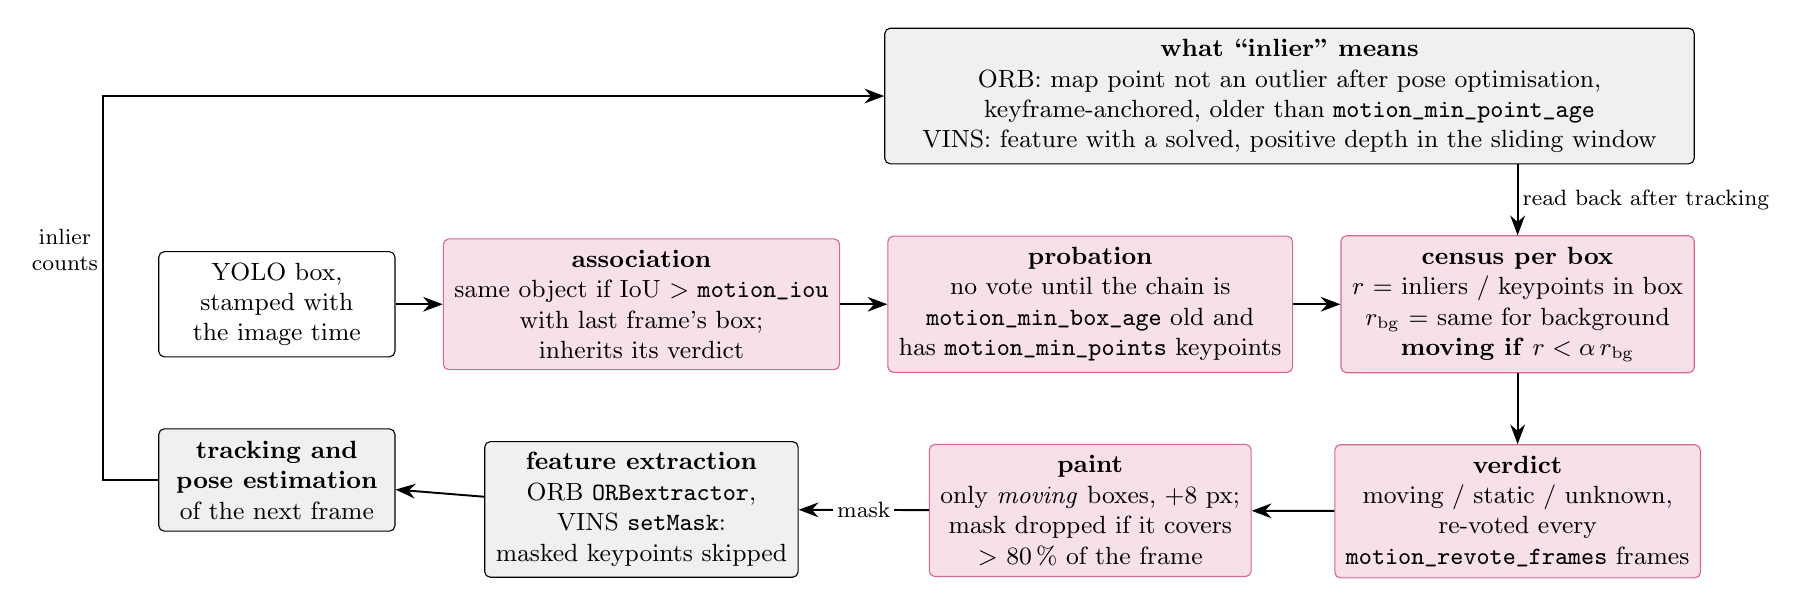
\begin{tikzpicture}[
      font=\small, node distance=9mm and 6mm,
      box/.style={draw, rounded corners=2pt, align=center, minimum height=13mm, minimum width=30mm, inner sep=4pt, fill=white},
      gate/.style={box, fill=purple!12, draw=purple!60},
      est/.style={box, fill=black!6},
      arr/.style={-{Stealth[length=2.5mm]}, line width=0.7pt},
      lbl/.style={font=\footnotesize, fill=white, inner sep=1.5pt}]
    % ---- row 1: from box to verdict
    \node[box] (yolo) {YOLO box,\\stamped with\\the image time};
    \node[gate, right=of yolo] (assoc) {\textbf{association}\\same object if IoU $>$ \repo{motion_iou}\\with last frame's box;\\inherits its verdict};
    \node[gate, right=of assoc] (probe) {\textbf{probation}\\no vote until the chain is\\\repo{motion_min_box_age} old and\\has \repo{motion_min_points} keypoints};
    \node[gate, right=of probe] (census) {\textbf{census per box}\\$r$ = inliers / keypoints in box\\$r_{\mathrm{bg}}$ = same for background\\\textbf{moving if} $r < \alpha\, r_{\mathrm{bg}}$};
    % ---- row 2: back to the tracker
    \node[gate, below=of census] (verdict) {\textbf{verdict}\\moving / static / unknown,\\re-voted every\\\repo{motion_revote_frames} frames};
    \node[gate, below=of probe] (paint) {\textbf{paint}\\only \emph{moving} boxes, +8 px;\\mask dropped if it covers\\$>$ 80\,\% of the frame};
    \node[est, below=of assoc] (extract) {\textbf{feature extraction}\\ORB \repo{ORBextractor},\\VINS \repo{setMask}:\\masked keypoints skipped};
    \node[est, below=of yolo] (track) {\textbf{tracking and}\\\textbf{pose estimation}\\of the next frame};
    % ---- row 0: where the inlier flag comes from (sits above probation+census)
    \node[est, anchor=south east, text width=100mm, minimum height=11mm] (src) at ($(census.north east)+(0,9mm)$)
      {\textbf{what ``inlier'' means}\\ORB: map point not an outlier after pose optimisation, keyframe-anchored, older than \repo{motion_min_point_age}\\VINS: feature with a solved, positive depth in the sliding window};
    % ---- arrows
    \draw[arr] (yolo) -- (assoc);
    \draw[arr] (assoc) -- (probe);
    \draw[arr] (probe) -- (census);
    \draw[arr] (src.south -| census.north) -- node[lbl, right] {read back after tracking} (census.north);
    \draw[arr] (census) -- (verdict);
    \draw[arr] (verdict) -- (paint);
    \draw[arr] (paint) -- node[lbl] {mask} (extract);
    \draw[arr] (extract) -- (track);
    \draw[arr] (track.west) -- ++(-7mm,0) |- node[lbl, pos=0.3, left, align=center] {inlier\\counts} (src.west);
  \end{tikzpicture}}
  \vspace{0.3ex}

  {\footnotesize Defaults: $\alpha = 0.5$, box age 30 frames, point age 30 frames (ORB), re-vote every 15 frames; the evaluation's best operating point was $\alpha = 0.25$. Only boxes judged \emph{moving} lose their features. 56\,\% of box-frames reached a vote; 13--16\,\% ended up masked.}
  \src{\repo{filter_motion.tex} chapter 3}
\end{frame}

\begin{frame}{3. \repo{filter_mode:=motion}: the gate cannot tell moving from stationary}
  \begin{columns}[T]
    \column{0.52\textwidth}
      \footnotesize ORB-SLAM3 census, \repo{dynamic_00_000}, ground-truth labelled box-frames
      \scriptsize\setlength{\tabcolsep}{3pt}
      \begin{tabular}{lrrrr}
        \toprule
        ratio $\le$ & moving flagged & static flagged & $J$ & AUC \\
        \midrule
        0.25 & 0.820 & 0.760 & +0.061 & 0.528 \\
        0.50 & 0.854 & 0.809 & +0.045 & \\
        0.75 & 0.875 & 0.840 & +0.035 & \\
        1.00 & 0.888 & 0.868 & +0.020 & \\
        \bottomrule
      \end{tabular}
      {\scriptsize 3\,307 moving and 1\,044 static box-frames; AUC 0.5 = coin toss. Older boxes score worse (AUC 0.40 at age 20).}
    \column{0.48\textwidth}
      \footnotesize VINS-Fusion, three census signals
      \scriptsize
      \begin{tabular}{lll}
        \toprule
        Signal & recall & false alarm \\
        \midrule
        solved depth & 0.25 & 0.23 \\
        reprojection residual & \multicolumn{2}{l}{\textbf{inverted}: movers score lower} \\
        residual availability & 0.56 & 0.41 \\
        \bottomrule
      \end{tabular}
      \vspace{0.6em}
      \footnotesize
      \begin{itemize}
        \item Every row flags stationary objects almost as often as moving ones
        \item Status: implemented in both pipelines, disabled by default; Exp.~3 reported on class mode
      \end{itemize}
  \end{columns}
  \src{\repo{exp3-motion-gate/motion_gate_summary.csv}, \repo{filter_motion.tex} table 4.2}
\end{frame}

\begin{frame}{3. Why: the census reads state the estimator has already cleaned}
  \footnotesize
  \begin{itemize}
    \item ORB-SLAM3 counts map points that survived \repo{TrackLocalMap}; points inconsistent with the optimised pose were marked outliers first. What is left inside a mover's box is whatever happened to fit, hence recall $\approx$ false alarm in every row of the previous slide
    \item VINS-Fusion \repo{outliersRejection} removes any feature above \SI{3}{px} reprojection error every frame; a mover's disagreeing features are gone within a frame or two, so the residual census measures survivors. That is why the residual signal came out \textbf{inverted}
    \item Test that confirms it: lowering \repo{min_dist} 30 $\to$ \SI{15}{px} tripled the features per box (coverage 19.6 $\to$ 55.8 \%), and the depth signal vanished: \SI{94.7}{\percent} of features inside moving objects held solved depths, 0 of 83 voted rows fell below threshold. More data, no signal
    \item A moving point triangulates to a wrong but valid depth; no depth test separates it
    \item Architectural, not tuning: no threshold on these quantities can repair it
  \end{itemize}
  \src{\repo{filter_motion.tex}, chapters 4--5}
\end{frame}


\begin{frame}{3. Where the gate reads, and where the evidence is lost}
  \centering
  \resizebox{0.98\textwidth}{!}{%
  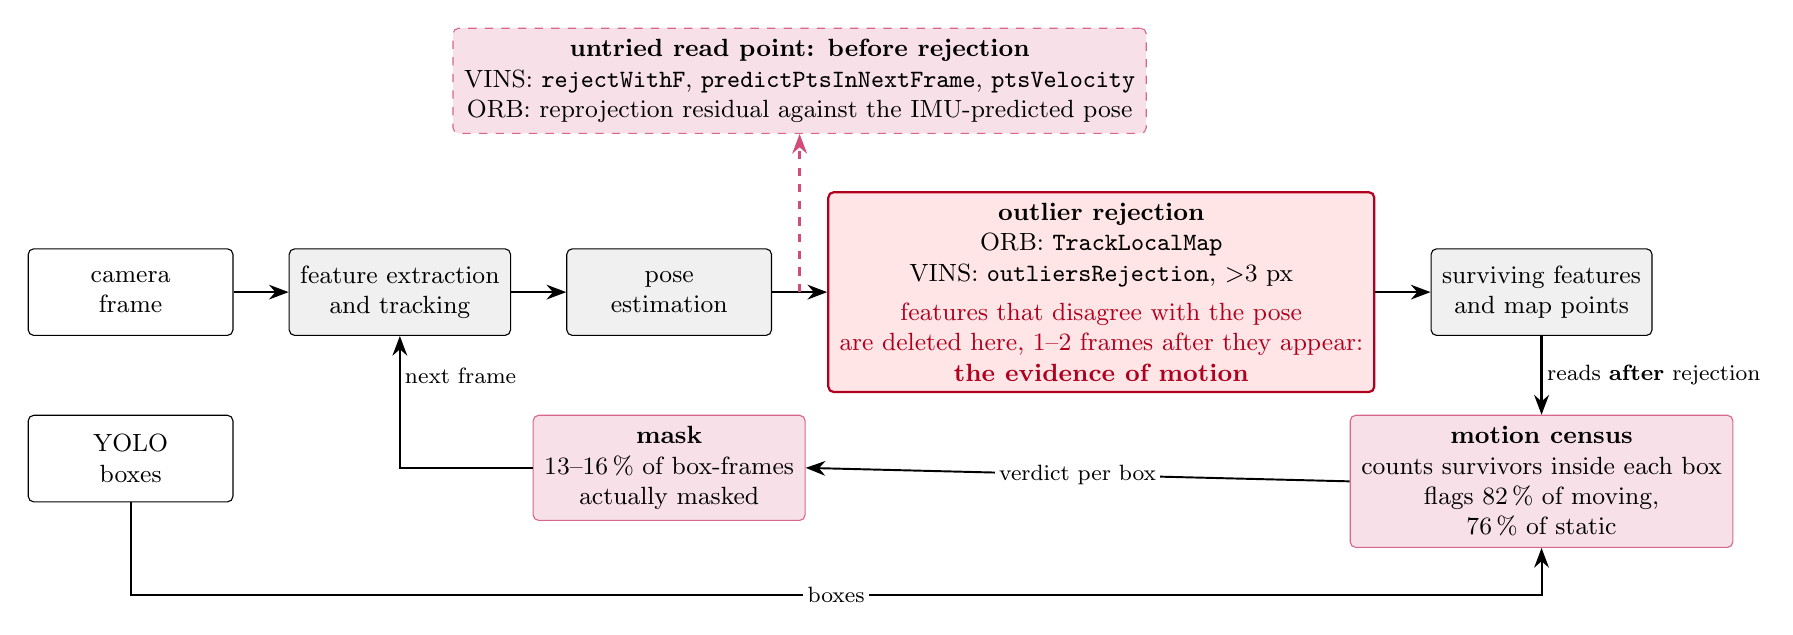
\begin{tikzpicture}[
      font=\small, node distance=10mm and 7mm,
      box/.style={draw, rounded corners=2pt, align=center, minimum height=11mm, minimum width=26mm, inner sep=4pt, fill=white},
      est/.style={box, fill=black!6},
      gate/.style={box, fill=purple!12, draw=purple!60},
      bad/.style={box, fill=red!10, draw=neg, line width=0.8pt},
      arr/.style={-{Stealth[length=2.5mm]}, line width=0.7pt},
      lbl/.style={font=\footnotesize, fill=white, inner sep=1.5pt}]
    % ---- row 1: estimator front end
    \node[box] (img) {camera\\frame};
    \node[est, right=of img] (feat) {feature extraction\\and tracking};
    \node[est, right=of feat] (pose) {pose\\estimation};
    \node[bad, right=of pose] (rej) {\textbf{outlier rejection}\\ORB: \repo{TrackLocalMap}\\VINS: \repo{outliersRejection}, $>$3 px\\[3pt]\textcolor{neg}{features that disagree with the pose}\\\textcolor{neg}{are deleted here, 1--2 frames after they appear:}\\\textcolor{neg}{\textbf{the evidence of motion}}};
    \node[est, right=of rej] (map) {surviving features\\and map points};
    % ---- row 2: detector (left), mask (middle), census (right, under the survivors)
    \node[box, below=of img] (yolo) {YOLO\\boxes};
    \node[gate, below=of pose] (mask) {\textbf{mask}\\13--16\,\% of box-frames\\actually masked};
    \node[gate, below=of map] (census) {\textbf{motion census}\\counts survivors inside each box\\flags 82\,\% of moving,\\76\,\% of static};
    % ---- arrows, row 1
    \draw[arr] (img) -- (feat);
    \draw[arr] (feat) -- (pose);
    \draw[arr] (pose) -- (rej);
    \draw[arr] (rej) -- (map);
    % ---- what the gate reads: survivors, after rejection
    \draw[arr, line width=1.1pt] (map.south) -- node[lbl, right] {reads \textbf{after} rejection} (census.north);
    % ---- detector boxes into the census, routed below row 2
    \draw[arr] (yolo.south) |- node[lbl, pos=0.75] {boxes} ($(census.south)+(0,-6mm)$) -- (census.south);
    % ---- census -> mask -> next frame
    \draw[arr] (census.west) -- node[lbl] {verdict per box} (mask.east);
    \draw[arr] (mask.west) -| node[lbl, pos=0.85, right] {next frame} (feat.south);
    % ---- the untried read point
    \coordinate (pre) at ($(pose.east)!0.5!(rej.west)$);
    \node[gate, dashed, minimum width=70mm] at ($(pre |- rej.north)+(0,14mm)$) (untried)
      {\textbf{untried read point: before rejection}\\VINS: \repo{rejectWithF}, \repo{predictPtsInNextFrame}, \repo{ptsVelocity}\\ORB: reprojection residual against the IMU-predicted pose};
    \draw[arr, dashed, purple!70, line width=0.9pt] (pre) -- (untried.south);
  \end{tikzpicture}}
  \vspace{0.5ex}

  {\footnotesize Grey: the estimator. Purple: what was built. Red: where the signal is destroyed. Dashed: where a motion signal can still exist.}
\end{frame}

\begin{frame}{3. What could work: signals taken \emph{before} rejection (untried, no data yet)}
  \footnotesize
  \begin{itemize}
    \item VINS: \repo{rejectWithF()}, RANSAC fundamental-matrix check, written but commented out; its outliers violate epipolar geometry by definition
    \item VINS: \repo{predictPtsInNextFrame()}, implemented, never called: predicted-vs-tracked displacement per feature
    \item VINS: \repo{ptsVelocity}, per-point image velocity already computed every frame; ego-motion is a smooth field, a mover a local anomaly
    \item ORB-SLAM3: reprojection residual of each keypoint against the IMU-predicted pose in \repo{Tracking}, before outlier marking
    \item Rule: nothing is quoted until \repo{analyse_motion_gate.py} has scored it against ground truth with the sample size stated (19 rows looked good, 1\,044 did not)
  \end{itemize}
\end{frame}

\begin{frame}{Next steps}
  \begin{enumerate}
    \item Rewrite Chapter 4 prose from the insight documents (tables and figures already regenerated)
    \item Quote planar ATE beside 3-D for the visual estimators
    \item Re-run \repo{realv3} on the 21 Oct extrinsics; measure the tracker lever arm
    \item Log per-box detector truth; re-score at a lower IoU
    \item Place \repo{map_03.db}; score \repo{map_02.db} with provenance stated
  \end{enumerate}
\end{frame}

\end{document}
